% ----------------------------------------------------
% Firmware Submodule
% ----------------------------------------------------
\documentclass[class=report,11pt,crop=false]{standalone}
% Page geometry
\usepackage[a4paper,margin=20mm,top=25mm,bottom=25mm]{geometry}

% Font choice
\usepackage{lmodern}

% \usepackage{lipsum}

% Use IEEE bibliography style
\bibliographystyle{IEEEtran}

% Line spacing
\usepackage{setspace}
\setstretch{1.20}

% Ensure UTF8 encoding
\usepackage[utf8]{inputenc}

% Language standard (not too important)
\usepackage[english]{babel}

% Skip a line in between paragraphs
\usepackage{parskip}

% For the creation of dummy text
\usepackage{blindtext}

% Math
\usepackage{amsmath}

% Header & Footer stuff
\usepackage{fancyhdr}
\pagestyle{fancy}
\fancyhead{}
\fancyhead[R]{\nouppercase{\rightmark}}
\fancyfoot{}
\fancyfoot[C]{\thepage}
\renewcommand{\headrulewidth}{0.0pt}
\renewcommand{\footrulewidth}{0.0pt}
\setlength{\headheight}{13.6pt}

% Epigraphs
\usepackage{epigraph}
\setlength\epigraphrule{0pt}
\setlength{\epigraphwidth}{0.65\textwidth}

% Colour
\usepackage{color}
\usepackage[usenames,dvipsnames]{xcolor}

% Hyperlinks & References
\usepackage{hyperref}
\definecolor{linkColour}{RGB}{77,71,179}
\hypersetup{
    colorlinks=true,
    linkcolor=linkColour,
    filecolor=linkColour,
    urlcolor=linkColour,
    citecolor=linkColour,
}
\urlstyle{same}

% Automatically correct front-side quotes
\usepackage[autostyle=false, style=ukenglish]{csquotes}
\MakeOuterQuote{"}

% Graphics
\usepackage{graphicx}
\graphicspath{{Images/}{../Images/}}
\usepackage{makecell}
\usepackage{transparent}

% SI units
\usepackage{siunitx}

% Microtype goodness
\usepackage{microtype}

% Listings
\usepackage[T1]{fontenc}
\usepackage{listings}
\usepackage[scaled=0.8]{DejaVuSansMono}

% Custom colours for listings
\definecolor{backgroundColour}{RGB}{250,250,250}
\definecolor{commentColour}{RGB}{73, 175, 102}
\definecolor{identifierColour}{RGB}{196, 19, 66}
\definecolor{stringColour}{RGB}{252, 156, 30}
\definecolor{keywordColour}{RGB}{50, 38, 224}
\definecolor{lineNumbersColour}{RGB}{127,127,127}
\lstset{
  language=Matlab,
  captionpos=b,
  aboveskip=15pt,belowskip=10pt,
  backgroundcolor=\color{backgroundColour},
  basicstyle=\ttfamily,%\footnotesize,        % the size of the fonts that are used for the code
  breakatwhitespace=false,         % sets if automatic breaks should only happen at whitespace
  breaklines=true,                 % sets automatic line breaking
  postbreak=\mbox{\textcolor{red}{$\hookrightarrow$}\space},
  commentstyle=\color{commentColour},    % comment style
  identifierstyle=\color{identifierColour},
  stringstyle=\color{stringColour},
   keywordstyle=\color{keywordColour},       % keyword style
  %escapeinside={\%*}{*)},          % if you want to add LaTeX within your code
  extendedchars=true,              % lets you use non-ASCII characters; for 8-bits encodings only, does not work with UTF-8
  frame=single,	                   % adds a frame around the code
  keepspaces=true,                 % keeps spaces in text, useful for keeping indentation of code (possibly needs columns=flexible)
  morekeywords={*,...},            % if you want to add more keywords to the set
  numbers=left,                    % where to put the line-numbers; possible values are (none, left, right)
  numbersep=5pt,                   % how far the line-numbers are from the code
  numberstyle=\tiny\color{lineNumbersColour}, % the style that is used for the line-numbers
  rulecolor=\color{black},         % if not set, the frame-color may be changed on line-breaks within not-black text (e.g. comments (green here))
  showspaces=false,                % show spaces everywhere adding particular underscores; it overrides 'showstringspaces'
  showstringspaces=false,          % underline spaces within strings only
  showtabs=false,                  % show tabs within strings adding particular underscores
  stepnumber=1,                    % the step between two line-numbers. If it's 1, each line will be numbered
  tabsize=2,	                   % sets default tabsize to 2 spaces
  %title=\lstname                   % show the filename of files included with \lstinputlisting; also try caption instead of title
}

% Caption stuff
\usepackage[hypcap=true, justification=centering]{caption}
\usepackage{subcaption}

% Glossary package
% \usepackage[acronym]{glossaries}
\usepackage{glossaries-extra}
\setabbreviationstyle[acronym]{long-short}

% For Proofs & Theorems
\usepackage{amsthm}

% Maths symbols
\usepackage{amssymb}
\usepackage{mathrsfs}
\usepackage{mathtools}

% For algorithms
\usepackage[]{algorithm2e}

% Spacing stuff
\setlength{\abovecaptionskip}{5pt plus 3pt minus 2pt}
\setlength{\belowcaptionskip}{5pt plus 3pt minus 2pt}
\setlength{\textfloatsep}{10pt plus 3pt minus 2pt}
\setlength{\intextsep}{15pt plus 3pt minus 2pt}

% For aligning footnotes at bottom of page, instead of hugging text
\usepackage[bottom]{footmisc}

% Add LoF, Bib, etc. to ToC
\usepackage[nottoc]{tocbibind}

% SI
\usepackage{siunitx}

% For removing some whitespace in Chapter headings etc
\usepackage{etoolbox}
\makeatletter
\patchcmd{\@makechapterhead}{\vspace*{50\p@}}{\vspace*{-10pt}}{}{}%
\patchcmd{\@makeschapterhead}{\vspace*{50\p@}}{\vspace*{-10pt}}{}{}%
\makeatother

% Tables
\usepackage{multirow}
\usepackage{longtable}
\usepackage{tabularx}
\makenoidxglossaries

\newacronym{radar}{RADAR}{Radio Detection and Ranging}
\begin{document}
\ifstandalone
\tableofcontents
\fi
% ----------------------------------------------------
\chapter{Camera/Transmitter (CT) \& Receiver (R) Hardware (PLLTHI032)\label{ch:hardware}}


\section{Subsystem introduction}\label{sc: HW_intro}
This section involves the design and implementation of the hardware for the transmitter/camera and receiver module for a Red-winged Starling nest monitoring system. The focus is to design a camera system that is motion activated when there is activity in the nest. This data is then transferred to a handheld receiver operated by the user on the ground. 

\section{Requirements \& Specifications}\label{sc: HW_R_S}
\begin{table}[h]
\centering
\begin{tabular}{|p{4cm}|p{5cm}|p{5cm}|p{1cm}|}
\hline
\textbf{User Requirements} & \textbf{Functional Requirements} & \textbf{Specifications} & \textbf{ATP} \\
\hline
Clear images of the birds must be captured and stored onboard. & The CT should be capable of capturing and storing quality images in all lighting conditions. & Camera should have infrared light, automated day/night mode switching, and fast onboard storage. & ATP1, ATP2 \\
\hline
The camera should only turn on with motion & The camera should trigger when there is movement. & Equip the CT with PIR sensors for motion detection. & ATP3 \\
\hline
The CT should transmit data wirelessly, avoiding cables & The CT should be capable of wireless data transmission. & The CT must be equipped with a working wireless module. & ATP1, ATP4 \\
\hline
The CT must be as small as possible. & The CT should not be too big as to disturb the birds. & The CT module must be no bigger than 60mm(W) x 80mm(L) x 60mm(H). & ATP5 \\
\hline
The Receiver must have wireless connectivity. & The receiver should be capable of establishing a wireless connection. & The receiver must be equipped with a wireless module. & ATP6 \\
\hline
The receiver must have onboard storage to store the retrieved data. & The receiver should be able to store the data onboard to be used later. & The receiver must have a MicroSD card option for storage. & ATP7 \\
\hline
The receiver must have a screen and interactive buttons to view the basic information. & The receiver should have buttons for easy navigation through the UI. & The receiver must be equipped with a screen and have 4 pushbuttons configure with internal pull up resistors. & ATP8 \\
\hline
\end{tabular}
\caption{User Requirements, Functional Requirements, Specifications, and ATP}
\label{tab:HW_Requirements}
\end{table}





\section{Design Process}\label{sc: HW_DP}

\subsection{Wired vs. Wireless Communication}
There are two options for communication: wired and wireless. the table below goes through the aspects of each. 

\begin{table}[h]
\centering
\begin{tabular}{|p{3.5cm}|p{6cm}|p{6cm}|}
\hline
\textbf{Aspect} & \textbf{Wired Communication} & \textbf{Wireless Communication} \\
\hline
Medium & Physical cables needed. & No physical cables, just radio signals. \\
\hline
Antenna & No need. & Needed for long distance data transfer. \\
\hline
Distance & Better for short distance. & Better for long distance. \\
\hline
Power Consumption & Lower due to cabling. & Higher due to antenna (active components). \\
\hline
Speed & Low latency – ideal for real-time applications. & Suitable for medium to high-speed data transfer. \\
\hline
Mobility & Limited with physical cables. & Free range in coverage area. \\
\hline
Security & Easy to damage physical cables. & Robust security protocols can be used. \\
\hline
Maintenance & High & Low \\
\hline
\end{tabular}
\caption{Comparison of Wired and Wireless Communication}
\label{tab:HW_communication_comparison}
\end{table}


With the nests located high up on buildings, wireless communication offers the user better access despite slightly slower speeds. The disadvantages of using wireless communication does not warrant a change to wired communication. 

\subsection{Wireless Communication Protocols}
There is no shortage of options when it comes to wireless communication protocols. The table below discusses the criterion upon which the different protocols were assessed on. 

\begin{table}[h]
\centering
\begin{tabular}{|p{4cm}|p{12cm}|}
\hline
\textbf{Criteria} & \textbf{Justification (Pass/Fail)} \\
\hline
Range \& Coverage & Can data be transmitted over a range of 10-15 m outdoors with minimal data loss? \\
\hline
Data Rate & Can higher data transfer rates be obtained (higher than 10 Mbps)? \\
\hline
Power Consumption & Is this protocol optimised to work well with low powered battery systems? \\
\hline
Latency & Does the protocol have a latency lower than 100ms? \\
\hline
Interference \& Noise & Is the protocol functional in crowded frequency bands? \\
\hline
Cost & Is this protocol affordable to design and maintain? \\
\hline
Payload & Is the protocol able to handle large data file transmission? \\
\hline
Existing Libraries \& Support & Does the protocol have available libraries and examples to use? Is there reliable developer support? \\
\hline
\end{tabular}
\caption{Criteria for Assessing Wireless Protocols}
\label{tab:HW_Comm_Criteria}
\end{table}

The criteria above will be used to grade each protocol with a pass or fail. The more passes a protocol has, the more likely it was to be chosen. 

\begin{table}[h]
\centering
\begin{tabular}{|l|l|l|l|l|l|l|}
\hline
\textbf{Criteria} & \textbf{BLE} & \textbf{Bluetooth Classic} & \textbf{ESP-Now} & \textbf{Wi-Fi} & \textbf{LoRa} & \textbf{RFID} \\
\hline
Range \& Coverage & \textcolor{red}{Fail} & \textcolor{red}{Fail} & \textcolor{ForestGreen}{Pass} & \textcolor{ForestGreen}{Pass} & \textcolor{ForestGreen}{Pass} & \textcolor{ForestGreen}{Pass} \\
\hline
Data Rate & \textcolor{red}{Fail} & \textcolor{red}{Fail} & \textcolor{red}{Fail} & \textcolor{ForestGreen}{Pass} & \textcolor{red}{Fail} & \textcolor{red}{Fail} \\
\hline
Power Consumption & \textcolor{ForestGreen}{Pass} & \textcolor{red}{Fail} & \textcolor{ForestGreen}{Pass} & \textcolor{red}{Fail} & \textcolor{ForestGreen}{Pass} & \textcolor{ForestGreen}{Pass} \\
\hline
Latency & \textcolor{red}{Fail} & \textcolor{ForestGreen}{Pass} & \textcolor{ForestGreen}{Pass} & \textcolor{ForestGreen}{Pass} & \textcolor{ForestGreen}{Pass} & \textcolor{ForestGreen}{Pass} \\
\hline
Interference \& Noise & \textcolor{ForestGreen}{Pass} & \textcolor{ForestGreen}{Pass} & \textcolor{ForestGreen}{Pass} & \textcolor{ForestGreen}{Pass} & \textcolor{red}{Fail} & \textcolor{red}{Fail} \\
\hline
Cost & \textcolor{ForestGreen}{Pass} & \textcolor{red}{Fail} & \textcolor{ForestGreen}{Pass} & \textcolor{ForestGreen}{Pass} & \textcolor{red}{Fail} & \textcolor{red}{Fail} \\
\hline
Payload & \textcolor{ForestGreen}{Pass} & \textcolor{ForestGreen}{Pass} & \textcolor{red}{Fail} & \textcolor{ForestGreen}{Pass} & \textcolor{red}{Fail} & \textcolor{red}{Fail} \\
\hline
Existing Libraries \& Support & \textcolor{ForestGreen}{Pass} & \textcolor{ForestGreen}{Pass} & \textcolor{ForestGreen}{Pass} & \textcolor{ForestGreen}{Pass} & \textcolor{ForestGreen}{Pass} & \textcolor{ForestGreen}{Pass} \\
\hline
\end{tabular}
\caption{Assessment of Different Wireless Protocols}
\label{tab:HW_Comm_Result}
\end{table}


Both WiFi and ESP-NOW emerged as viable options from this evaluations, with the fewest fails of all the options. Looking at the fails of ESP-NOW, it has an very low payload of around 250 bytes, making it capable of sending only messages between boards. The data rate is around 1 Mbps, which is okay, but not as fast as WiFi. 
WiFi, on the other hand, only has issues with power consumption. With the high speed data transfer and lower latency relative to the other options, this is an acceptable trade off. While yes, there are other options that offer lower power consumption, the data transfer is also slower. Looking at the bigger picture, if the data rate is slower, despite having a lower power consumption, the module will have to stay on for longer till the transfer is complete. This could consume even more power than WiFi, since the module would not have to stay on for that much longer. 
The user also does not want to wait a very long time to retrieve the data. Their time is important. WiFi is chosen. The next part of the design process looks at the different micro-controller options. 

\subsection{Transmitter Microcontroller}

There are millions of different WiFi microcontrollers to choose from in the market, ranging from Arduino, ESP, NRF Dev boards, Raspberry Pi Pico W, and ST Micron Dev boards. However, the NRF boards are extremely expensive, and only offer BLE communication, not to mention minimal customer support. The Arduino board options, like the nano 33 IOT and UNO Wi-Fi, are expensive and bulky respectively. The ST Micro Dev Boards are also quite costly in their own regard, since all the affordable options have been sold out, like the STM32F401, but one would need to look at external Wi-Fi modules since those are sold separately. This leaves the Raspberry Pi Pico W and ESP boards. The table below will lay out a set of criteria that different boards will be assessed on to see which one would be suitable to fulfill the needs of the transmitter.

\begin{table}[h]
\centering
\begin{tabular}{|l|p{10cm}|}
\hline
\textbf{Criteria} & \textbf{Justification} \\
\hline
Processing Power & Does the microcontroller have enough processing power in terms of the number of cores and clock speed (~240 MHz)? \\
\hline
Memory & Is there enough RAM and flash memory to handle tasks related to handling images? \\
\hline
Low Power Modes & Does the microcontroller have low power standby modes available? \\
\hline
Power Consumption & Is the microcontroller power efficient in active mode? \\
\hline
Input/Output (I/O) Pins & Can the microcontroller support external peripherals with available I/O pins? \\
\hline
Development Environment & Are there enough tools available to assist with development? \\
\hline
Cost & Is the microcontroller affordable? \\
\hline
Size & Is the microcontroller small and compact? \\
\hline
\end{tabular}
\label{tab:HW_CT_Criteria_1}
\end{table}

\begin{table}[h]
\centering
\begin{tabular}{|l|p{10cm}|}
\hline
\textbf{Criteria} & \textbf{Justification} \\
\hline
Existing Libraries \& Support & Does the microcontroller have many libraries available and community support? \\
\hline
Operating Voltage & Is the operating voltage of the microcontroller 5V? \\
\hline
Camera Support & Does this microcontroller have good support with regards to camera attachments? \\
\hline
Weight & Does the microcontroller weigh more than 30 g? \\
\hline
MicroSD card holder & Does the microcontroller have a microSD card holder onboard \\
\hline
\end{tabular}
\caption{Criteria for the Transmitter Microcontroller Selection}
\label{tab:HW_CT_Criteria_2}
\end{table}


The table below proceeds to assess four potential board which have been chosen for the transmitter submodule against the criterion outlines in Table 1.5.

\begin{table}[h]
\centering
\begin{tabular}{|p{3.5cm}|l|l|l|l|l|}
\hline
\textbf{Criteria} & \textbf{Pi Pico W} & \textbf{ESP32-CAM} & \textbf{ESP32-CH340} & \textbf{ESP32-C6} & \textbf{ESP32 S3} \\
\hline
Processing Power & \textcolor{red}{Fail} & \textcolor{ForestGreen}{Pass} & \textcolor{ForestGreen}{Pass} & \textcolor{red}{Fail} & \textcolor{ForestGreen}{Pass} \\
\hline
Memory & \textcolor{ForestGreen}{Pass} & \textcolor{ForestGreen}{Pass} & \textcolor{ForestGreen}{Pass} & \textcolor{ForestGreen}{Pass} & \textcolor{ForestGreen}{Pass} \\
\hline
Low Power Modes & \textcolor{ForestGreen}{Pass} & \textcolor{ForestGreen}{Pass} & \textcolor{ForestGreen}{Pass} & \textcolor{ForestGreen}{Pass} & \textcolor{ForestGreen}{Pass} \\
\hline
Power Consumption & \textcolor{ForestGreen}{Pass} & \textcolor{ForestGreen}{Pass} & \textcolor{red}{Fail} & \textcolor{ForestGreen}{Pass} & \textcolor{red}{Fail} \\
\hline
Input/Output (I/O) Pins & \textcolor{ForestGreen}{Pass} & \textcolor{red}{Fail} & \textcolor{ForestGreen}{Pass} & \textcolor{ForestGreen}{Pass} & \textcolor{ForestGreen}{Pass} \\
\hline
Development Environment & \textcolor{ForestGreen}{Pass} & \textcolor{ForestGreen}{Pass} & \textcolor{ForestGreen}{Pass} & \textcolor{ForestGreen}{Pass} & \textcolor{ForestGreen}{Pass} \\
\hline
Cost & \textcolor{ForestGreen}{Pass} & \textcolor{ForestGreen}{Pass} & \textcolor{ForestGreen}{Pass} & \textcolor{red}{Fail} & \textcolor{ForestGreen}{Pass} \\
\hline
Size & \textcolor{ForestGreen}{Pass} & \textcolor{ForestGreen}{Pass} & \textcolor{red}{Fail} & \textcolor{red}{Fail} & \textcolor{ForestGreen}{Pass} \\
\hline
Existing Libraries \& Support & \textcolor{ForestGreen}{Pass} & \textcolor{ForestGreen}{Pass} & \textcolor{ForestGreen}{Pass} & \textcolor{ForestGreen}{Pass} & \textcolor{ForestGreen}{Pass} \\
\hline
Operating Voltage & \textcolor{ForestGreen}{Pass} & \textcolor{ForestGreen}{Pass} & \textcolor{ForestGreen}{Pass} & \textcolor{ForestGreen}{Pass} & \textcolor{ForestGreen}{Pass} \\
\hline
Camera Support & \textcolor{ForestGreen}{Pass} & \textcolor{ForestGreen}{Pass} & \textcolor{ForestGreen}{Pass} & \textcolor{red}{Fail} & \textcolor{red}{Fail} \\
\hline
Weight & \textcolor{ForestGreen}{Pass} & \textcolor{ForestGreen}{Pass} & \textcolor{ForestGreen}{Pass} & \textcolor{ForestGreen}{Pass} & \textcolor{ForestGreen}{Pass} \\
\hline
MicroSD card holder & \textcolor{red}{Fail} & \textcolor{ForestGreen}{Pass} & \textcolor{red}{Fail} & \textcolor{red}{Fail} & \textcolor{red}{Fail} \\
\hline
\end{tabular}
\caption{Assessment of Different Transmitter Microcontrollers}
\label{tab:HW_CT_Result}
\end{table}

The Pi Pico W and ESP32-CH340 have poor processing power and power consumption respectively, with the latter having an additional space constraint. The ESP32-C8 had similar limitations, while also being expensive with poor camera support. The ESP32 S3 lacks camera support and has bad power consumption. 

The ESP32-CAM stands out, offering an onboard MicroSD card holder with quad SPI and camera, with support for external antenna. While there are fewer GPIO pins available for external devices, the trade-offs with the other boards are far worse, since the other options would need an external camera and MicroSD card. This would increase power consumption, cost and reduces the GPIO pins available. The ESP32-CAM avoids these issues, which is why it was chosen. 


\subsection{Receiver Microcontroller}

Table \ref{tab:HW_Requirements} detailed what the Receiver module should have. The table below lays out a set of criteria to assess different microcontroller options. However, since the microcontroller options have already been assessed in the previous section, just a few of the amended criteria will be looked at. 

\begin{table}[h]
\centering
\begin{tabular}{|l|p{10cm}|}
\hline
\textbf{Criteria} & \textbf{Justification} \\
\hline
Processing Power & Does the microcontroller have enough processing power in terms of the number of cores and clock speed (~100 MHz)? \\
\hline
Memory & Is there enough RAM and flash memory to handle image transfer? \\
\hline
Input/Output (I/O) Pins & Are there enough GPIO pins on the microcontroller to support a screen (I2C) and MicroSD card (SPI)? \\
\hline
Cost & Is the microcontroller affordable? \\
\hline
Size & Is the microcontroller small and compact? \\
\hline
Weight & Does the microcontroller weigh more than 5 g? \\
\hline
\end{tabular}
\caption{Criteria for Receiver Microcontroller Selection}
\label{tab:HW_R_Criteria}
\end{table}

Using table \ref{tab:HW_R_Criteria}, three microcontrollers from table \ref{tab:HW_CT_Criteria} are assessed to see if they meet the demands of this module.

\begin{table}[h]
\centering
\begin{tabular}{|l|l|l|l|}
\hline
\textbf{Criteria} & \textbf{Pi Pico W} & \textbf{ESP32-C6} & \textbf{ESP32 S3} \\
\hline
Processing Power & \textcolor{ForestGreen}{Pass} & \textcolor{ForestGreen}{Pass} & \textcolor{ForestGreen}{Pass} \\
\hline
Memory & \textcolor{ForestGreen}{Pass} & \textcolor{ForestGreen}{Pass} & \textcolor{ForestGreen}{Pass} \\
\hline
Input/Output (I/O) Pins & \textcolor{ForestGreen}{Pass} & \textcolor{ForestGreen}{Pass} & \textcolor{ForestGreen}{Pass} \\
\hline
Cost & \textcolor{ForestGreen}{Pass} & \textcolor{red}{Fail} & \textcolor{ForestGreen}{Pass} \\
\hline
Size & \textcolor{ForestGreen}{Pass} & \textcolor{red}{Fail} & \textcolor{ForestGreen}{Pass} \\
\hline
Weight & \textcolor{ForestGreen}{Pass} & \textcolor{red}{Fail} & \textcolor{red}{Fail} \\
\hline
\end{tabular}
\caption{Assessment of Different Receiver Microcontrollers}
\label{tab:HW_R_Result}
\end{table}

This was an easy decision. The Pi Pico W was the smallest, cheapest, and lightest microcontroller option. It had the best price to performance ratio, hence why it is chosen to operate the receiver module. 

\subsection{Miscellaneous Parts}
\begin{itemize}
    \item PIR Sensors: It would be power inefficient if the ESP32 CAM were on all the time. To solve this, the Mini PIR Sensor (HC-SR505) was picked since it had a 100 degree detection angle, and low quiescent current (low power consumption). The transmitter module will be equipped with two of these. An OR gate will combine their output that is sent to the microcontroller to reduce the GPIO pins used. details on that circuit in the design section. 
    \item Infrared Lights: This is needed for the images captured at night to be visible. There are two different wavelengths to choose from; 850 nm and 940 nm. While 850nm deliver exceptional images in lowlight conditions but gives off a bright red glow when on. 940 nm is a more viable option if minimal invasion is required, i.e., the requirements of this product. Despite delivering lower image quality, there is no visible light that may disturb the birds. Therefore, 940 nm IR LEDs were picked for this product. It might be difficult to test if a 940 nm IR LED works since this light is beyond the visible spectrum. Just make sure the voltage drop is 1.1 V and the current draw is around 50 mA. 
    \item 433MHz RF Link Kit: When the transmitter is in sleep mode, the WiFi module is inactive, so the receiver will not be able to establish a WiFi connection. This component has its own receiver and transmitter. The receiver pulls the GPIO pin that the RF transmitter is connected to high when there is no connection. This pings the RF receiver, which is connected to a pin on the transmitter. Both RF transmitter and receiver are powered with 5V. The data pins (connected to the microcontrollers) output a 3V3 signal when high and 0V when low. 
    \item MicroSD card (SPI): This is needed for the receiver since the Pi Pico W does not have a built-in MicroSD card. The microcontroller only supports normal SPI, not quad SPI like the ESP32-CAM. A simple module with 6 pins: (1)VCC, (2)GND, (3)CS, (4)CLK, (5)MOSI, and (6)MISO was purchased. The module needs 3V3 power. 
    \item Display (I2C): The information the user needs can be shown on a 16x2 liquid crystal display. Four pushbuttons are used to interact with the display. Each button is configured with an internal pull-up resistor. The screen connects to the Pi using I2C, and is powered by 3V3. 
\end{itemize}

\section{Final Design}\label{sc: HW_FD}

\subsection{General Overview}
\begin{figure}[h]
\centering
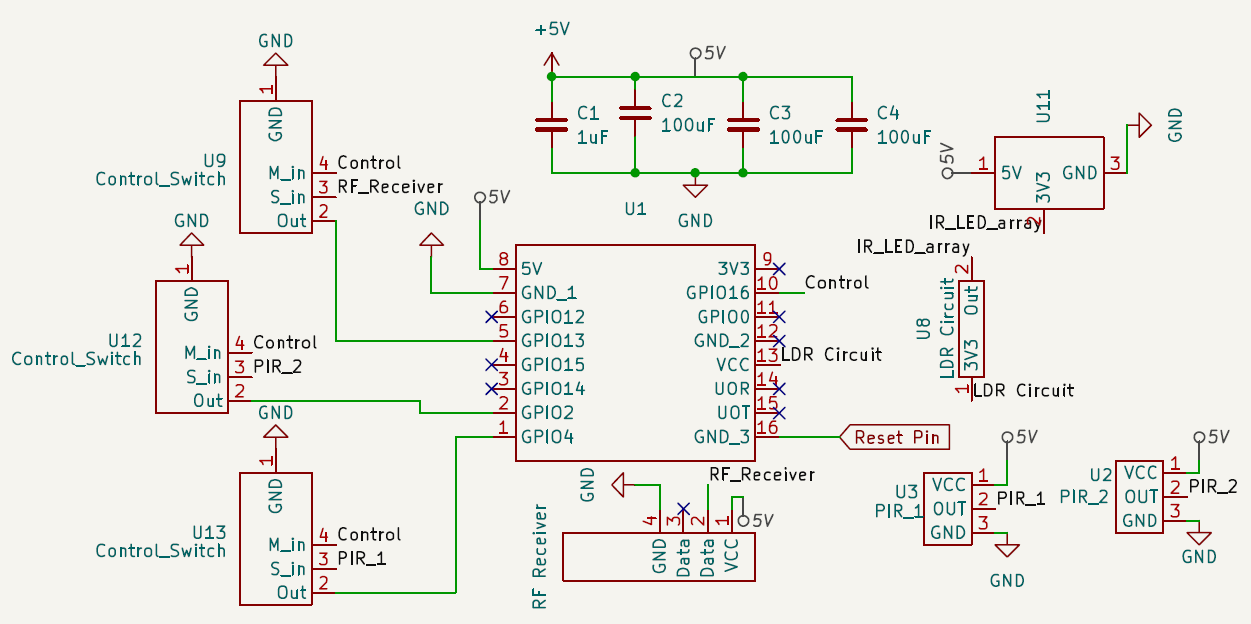
\includegraphics[width=0.7\textwidth]{Images/Transmitter_layout.png}
\caption{Final Transmitter Board Layout}
\label{fig:T_Schem}
\end{figure}

In the transmitter, shown in Figure \ref{fig:T_Schem}, the ESP32-CAM, powered by 5VDC. is the main hub that houses the connections for the LDR circuit, IR LED array, PIR sensors, and RF receiver. 
Given the limited GPIO pins, which become unusable when the WiFi module or MicroSD card are active, the PIR sensors and RF receiver are connected to Real-Time Clock (RTC) pins. These are the only pins that wake up the ESP32-CAM from deep sleep. 

When either of the two PIR sensors detect motion, the ESP32-CAM is activated (through PNP switches), which turns on the LDR circuit (through the VCC pin); if it is dark, the IR LED circuit turns on to light up the area. GPIO1, which is fed to the base of the PNP switch, would go high as soon as the ESP32-CAM is activated, to prevent the board from shorting the sensors. The OV2640 camera is a 2MP camera with a maximum resolution of 1280x720. The IR filter present in the lens was challenging to remove. 

When the RF Receiver goes high from the user sending a signal from the RF transmitter, the ESP32-CAM is activated for data transmission. The same PNP switch as used for the PIR connections was used here. 

The storage is limited to 4GB. The HC MicroSD card must be formatted to FAT32. The RF receiver wakes the ESP32-CAM out of deep sleep mode for data retrieval (since WiFi also becomes inactive). 

\begin{figure}[h]
\centering
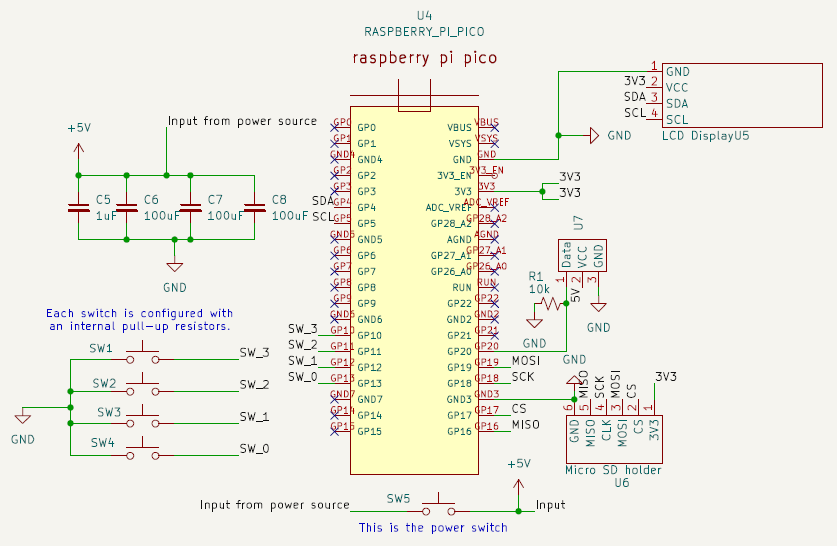
\includegraphics[width=0.7\textwidth]{Images/Receiver_layout.png}
\caption{Final Receiver Board Layout}
\label{fig:R_Schem}
\end{figure}

In the receiver, shown in Figure \ref{fig:R_Schem}, the Pi Pico W is the main hub connecting various peripherals:
\begin{itemize}
    \item Liquid Crystal Display: The module connects to the Pi Pico W with I2C protocol. The GPIO4 and GPIO5 pins are connected to SDA and SCL respectively. The 3V3 pin and GND pins are connected to the VCC and Ground pins of the display. 
    \item SD Card Reader: The module connects to the Pi Pico W with SPI protocol. 
    \item Pushbuttons: Allow for the user to interface with the display. These buttons are connected to GPIO10-13. 
    \item RF Transmitter: The data line connects to GPIO20 on the Pi Pico W. When the WiFi connection cannot be established between the Pi Pico W and the ESP32-CAM, then GPIO20 is set high to activate the ESP32-CAM on remotely. 
\end{itemize}



\subsection{Transmitter Support Circuitry and Testing}

\begin{figure}[hbt!]
    \begin{subfigure}[b]{0.25\textwidth}
        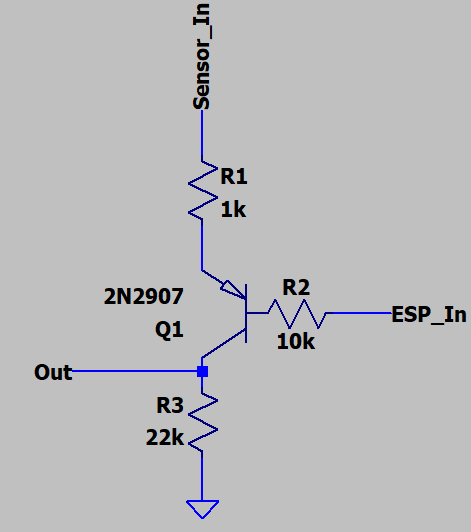
\includegraphics[width=\linewidth]{Images/Switch_circuit.png}
        \caption{PNP Switch Schematic}
        \label{fig:PNP_Switch}
    \end{subfigure}
    \hfill
    \begin{subfigure}[b]{0.4\textwidth}
        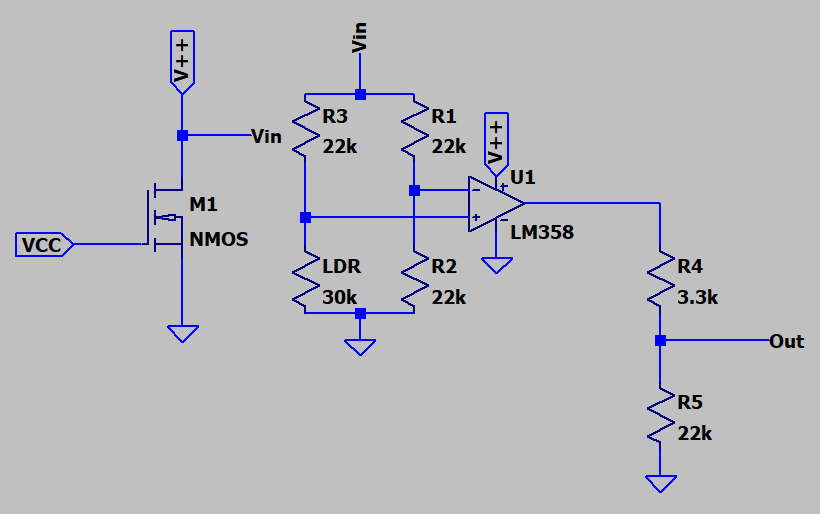
\includegraphics[width=\linewidth]{Images/LDR_circuit.png}
        \caption{LDR Comparator Circuit Schematic}
        \label{fig:LDR_schem}
    \end{subfigure}
    \hfill
    \begin{subfigure}[b]{0.25\textwidth}
        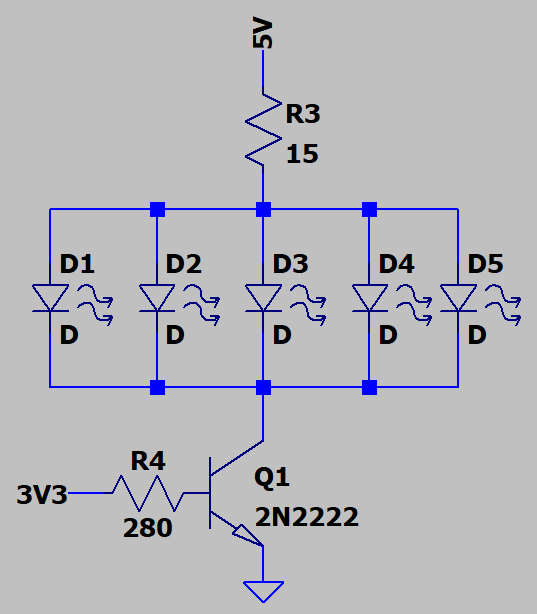
\includegraphics[width=\linewidth]{Images/IR_LED_Array.png}
        \caption{IR LED Array Schematic}
        \label{fig:LED_schem}
    \end{subfigure}
\end{figure}

Figure \ref{fig:PNP_Switch} shows a 2N2907 transistor acting as a buffer between the sensor and GPIO pins. A resistor is placed between the Sensor and the emitter to prevent current overload. The collector is connected to the GPIO pin with a resistor pulling the pin to GND. The base is connected to GPIO16 through a 10k resistor. 

When GPIO16 is low, the sensor input is allowed to trigger the GPIO pin. When the sensor input is high, the ESP32-CAM is woken up from deep sleep, and GPIO16 is immediately set to high, to isolate the sensor from the GPIO pin. 

The simulated output was around 3V, which was confirmed in testing when a simulated 3V3 input was applied to the switch, and the base was controlled by a 3V3 voltage. The GPIO pin will still trigger a high since the quoted GPIO range on the ESP datasheet is 2.3V to 3.6V. 

Figure \ref{fig:LDR_schem} shows a basic comparator circuit. The Light Dependent Resistor (LDR) was test under dark conditions, having a resistance of 25k, which dropped in light conditions to 6.5k. The inverting (-) and non-inverting (+) pins are connected to voltage dividers. The (-) pin is connected to 2.5V. The (+) pin is connected to a voltage divider with the LDR. When the surroundings get darker, the resistance increases and the voltage at the (+) increases. Once (V+)>(V-), the output, fed through another voltage divider, will be 3V3. Otherwise the output will be around 0V (22 mV). 

An N-Channel MOSFET is used as a level shift, such that when the 3V3 voltage from the ESP32-CAM is applied to it, the rest of the circuit can then be supplied with 5V, otherwise the circuit is inactive.

Figure \ref{fig:LED_schem} shows a 2N2222 transistor acts as a switch to control the flow of current to 5 IR LEDs are placed in parallel. The switch is operated by the comparator output, i.e., the output from the LDR circuit. When the base is high (3V3), current flows through the LEDs, otherwise, the switch will be off and no current will flow. 

The datasheet quoted that each 950nm LED required 1.1V and 50mA. The circuit was simulated and built to deliver each LED with rated power. Lab testing confirmed that each LED drew 48mA. The emitting light from these LEDs are invisible to the human eye. Normal green LEDs were used to test if the switch was working. The resistor values were adjusted to ensure the rated current was applied to each LED. The circuit functioned perfectly. 

The IR LEDs and corresponding resistors were placed in the circuit and run for 10 minutes with the rated power. The current and voltage remained stable, with the current and voltage across the IR LEDs remaining constant. There was heat being radiated off each LED, which was normal. 

\section{Power Consumption}\label{sc: HW_PC}
\subsection{Transmitter Power Consumption}
Now that the supporting circuits have been constructed, it is time to do an evaluation of the power consumption of the transmitter when the ESP32-CAM is in deep sleep and active mode. 


\begin{table}[h]
\centering
\begin{tabular}{|p{2.5cm}|p{6.5cm}|p{6.5cm}|}
\hline
\textbf{Device} & \textbf{Power Consumption in Deep Sleep} & \textbf{Power Consumption in Active Mode} \\
\hline
ESP32-CAM & 6 mA @ 5 V & 180 mA @ 5 V \\
\hline
PNP Switch & 0 mA @ 0 V & When Sensor input goes high: 0.133 mA @ 5 V \\
& & When base current is applied: 3.31 pA @ 5V \\
\hline
RF Receiver & When output low: 4 mA @ 5 V & When output low: 4 mA @ 5 V \\
& When output high: 20 mA @ 5 V & When output high: 20 mA @ 3.4 V \\
\hline
PIR (x2) & 0.06 mA @ 5 V & 0.06 mA @ 5 V \\
\hline
LDR Circuit & 0 mA @ 0 V & When light: 0.34 mA @ 5V \\
& & When dark: 0.6 mA @ 5V \\
\hline
IR LED Array & 0 mA @ 5 V & When LDR out low: 0 mA @ 5 V \\
& & When LDR out high: 262 mA @ 5 V \\
\hline
Total & Min: 10.06 mA @ 5 V, 50.3 mW & Min: 184.40 mA @ 5 V, 922 mW \\
& Max: 26.06 mA @ 5 V, 130.3 mW & Max: 462.53 mA @ 5 V, 2.31 W \\
\hline
\end{tabular}
\caption{Transmitter Power Consumption}
\label{tab:CT_PWR}
\end{table}

The power consumption reaches a high of 2.31 W when the camera, WiFi and SD card is in use. This should be avoided as much as possible to increase the longevity of the battery onboard. In standby mode, the system performs great by consuming very little power which will help save battery in periods when there is no nest activity. 

\subsection{Receiver Power Consumption}
The receiver will always remain in the active mode. When the user no longer needs to use the Receiver, they can just turn it off. 

\begin{table}[h]
\centering
\begin{tabular}{|l|l|}
\hline
\textbf{Device} & \textbf{Power Consumption in Active Mode} \\
\hline
Pi Pico W & 60 mA @ 5 V \\
\hline
LCD Display & 30 mA @ 3V3 \\
\hline
RF Transmitter & When on standby: 0 mA @ 5 V \\
& When in use: 4 mA @ 5 V \\
\hline
MicroSD Card Holder & 16 mA @ 3V3 \\
\hline
Total & Min: 106 mA @ 5 V, 530 mW \\
& Max: 110 mA @ 5 V, 550 mW \\
\hline
\end{tabular}
\caption{Receiver Power Consumption}
\label{tab:R_PWR}
\end{table}

Power consumption is fairly consistent. These values were calculated when the WiFi module was in operation, so this is possibly the highest power consumption that could be seen on the receiver. 

\section{Testing and Results} \label{sc: HW_TR}
\subsection{Acceptance Test Procedures}

\begin{table}[h]
\centering
\begin{tabular}{|p{1cm}|p{15cm}|}
\hline
\textbf{Code} & \textbf{Description} \\
\hline
ATP1 & Test that the camera can take clear images and store it onboard.\\
\hline
ATP2 & Test the night vision capabilities of the camera module. \\
\hline
ATP3 & Test that the ESP32-CAM wakes up from deep sleep when the PIR picks up motion. \\ 
\hline
ATP4 & Test that the RF receiver pulls the pin on the ESP32-CAM it is connected to high when the RF transmitter is fed a pulse.\\ 
\hline
ATP5 & Test that the CT module can fit in the space constraint. \\
\hline
ATP6 & Initialise a Wi-Fi hotspot on the Pi Pico W to test the module. \\ 
\hline
ATP7 & Test the MicroSD card module.\\ 
\hline
ATP8 & Test if the screen can display text. \\ 
\hline
\end{tabular}
\caption{Table of ATP Descriptions}
\label{tab:ATPs_Criteria}
\end{table}

Below are all the test scripts that will be used in the ATPs. These can be found in the GitHub under "Sample Code":

"ATP1.ino": Create a WiFi hotspot with ssid "ESP\_WiFi" and password "Thiyashan" on your device. Go to Tools>Serial Monitor to get the IP address of the board and input this to the browser on your device. The HTTP server should display with three buttons: ROTATE, CAPTURE PHOTO and REFRESH PAGE, as shown in \ref{fig:ATP1_Test}. Press CAPTURE PHOTO which saves the image to the SD card. Wait 5 seconds then press REFRESH PAGE. If the image displays, then the test passed. Once the test is completed, close application. \cite{randomnerdtutorialsESP32CAMTake}

\begin{figure}[h]
\centering
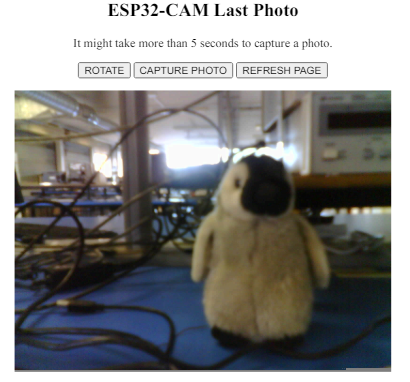
\includegraphics[width=0.4\textwidth]{Images/ATP1.png}
\caption{HTTP Web Page Layout With Image Displayed}
\label{fig:ATP1_Test}
\end{figure}

"ATP6.ino": Once the program is loaded onto the Pi Pico W, open Tools>Serial Monitor and change the baud rate to 115200. Open the WiFi setting on your device, and wait around 10s for "Pi\_WiFi" to appear. Enter password "Thiyashan" if you wish to connect. If the network appears, the it is a pass. Close all applications after test.

"ATP7.ino": The MISO, MOSI, SC, and SCK pins are connected to 16, 19, 17, 18 respectively and initialised as such in the code. Place an SD card with no files into the holder. Run program. This should load a text file called "example.txt". Unplug the SD card and read it on your computer to make sure the text file was generated. If it is there, then the system has passed the ATP. 

"ATP8.ino": Wait around 5 seconds for the message "Hello World" to be displayed on the screen. If this happens, then the screen passes the ATP. 

There are three possible results in table \ref{tab:ATPs_result}. Either a Pass, Fail or Time. Pass and Fail is with regards to the designs ability to satisfy a user requirement. Time means that there was not enough time to fully test the ATP, so the design could pass the ATP if there was sufficient time. 

\begin{table}[h]
\centering
\begin{tabular}{|p{1cm}|p{13cm}|p{2cm}|}
\hline
\textbf{Code} & \textbf{Acceptance Criterion} & \textbf{Result} \\
\hline
ATP1 & The pictures that are taken should be clear at 1m. Load test script "ATP1.ino" and follow the instructions above. & Pass \\
\hline
ATP2 & Place the camera in a dark area to test camera quality. Load test script "ATP1.ino" onto the ESP32-CAM to view the images. & Time* \\
\hline
ATP3 & The PIR must output 3V3 to the GPIO pin it is connected to. When motion stops, it should take around 10s for the voltage to return to zero. The components passes if this happens & Pass \\ 
\hline
ATP4 & When a 3V3 pulse is fed to the RF transmitter, the oscilloscope, set to trigger a rising edge, must detect a 3V3 pulse on the RF receiver. The component passes if this happens & Pass \\ 
\hline
ATP5 & An 60mm(W) x 80mm(L) x 60mm(H) box was constructed out of paper to see if the module fits in the space. If all components fit then it is a pass. & Pass \\
\hline
ATP6 & Load test script "ATP6.ino" onto the Pi Pico W. Once loaded, follow the instructions below the table. & Pass \\ 
\hline
ATP7 & Follow the instruction in "ATP7.ino". & Pass \\ 
\hline
ATP8 & Load test script "ATP8.ino" onto the Pi Pico W and follow the instructions above. & Pass \\ 
\hline
\end{tabular}
\caption{Table of ATP results}
\label{tab:ATPs_result}
\end{table}

* ATP2 failed on time. When purchasing the ESP32-CAM, it was expected that the IR filter was easily removable by opening the lens and popping it out. However, position was relocated in this model to the base of the camera. Accessing it required fully disassembling and desoldering the camera with the risk of permanent damage. With more time this could be completed, or alternatively an older camera model could be purchased but there were not any available that could be purchased before the deadline. 

\section{Conclusion} \label{sc: HW_C}
This subsection was successful in designing a working receiver and camera/transmitter module for the Red Winged Starling nest monitoring system. The design process was thorough, where each decision was graded in 
a pass/fail system to assess whether it was a viable option or not. 

The ESP32-CAM and Pi Pico W were the main hub for the receiver and transmitter in the final design respectively, since each showcased a balance between cost and performance in the grading system. 

The system was built with motion-activated capture and wireless data transfer in mind, while also prioritising power efficiency and cost. The hardware was tested to ensure all components met a set of criteria. Despite the limitations, the design was efficient in the end. 

The design provided insights into the trade-offs that need to be made in order to cater for the specific user needs, as well as future improvements that could be made, such as adding video capabilities and mending the night vision abilities. 

% ----------------------------------------------------
\ifstandalone
\bibliography{../Bibliography/References.bib}
\printnoidxglossary[type=\acronymtype,nonumberlist]
\fi
\end{document}
% ----------------------------------------------------